\documentclass[12pt]{article}
\usepackage{graphicx}
%\documentclass[journal,12pt,twocolumn]{IEEEtran}
\usepackage[none]{hyphenat}
\usepackage{graphicx}
\usepackage{listings}
\usepackage[english]{babel}
\usepackage{graphicx}
\usepackage{caption}
\usepackage{hyperref}
\usepackage{booktabs}
\def\inputGnumericTable{}
\usepackage{color}                                            %%
    \usepackage{array}                                            %%
    \usepackage{longtable}                                        %%
    \usepackage{calc}                                             %%
    \usepackage{multirow}                                         %%
    \usepackage{hhline}                                           %%
    \usepackage{ifthen}
\usepackage{array}
\usepackage{amsmath}   % for having text in math mode
\usepackage{listings}
\lstset{
language=tex,
frame=single,
breaklines=true
}

%Following 2 lines were added to remove the blank page at the beginning
\usepackage{atbegshi}% http://ctan.org/pkg/atbegshi
\AtBeginDocument{\AtBeginShipoutNext{\AtBeginShipoutDiscard}}
%


%New macro definitions
\newcommand{\mydet}[1]{\ensuremath{\begin{vmatrix}#1\end{vmatrix}}}
\providecommand{\brak}[1]{\ensuremath{\left(#1\right)}}
\providecommand{\norm}[1]{\left\lVert#1\right\rVert}
\newcommand{\solution}{\noindent \textbf{Solution: }}
\newcommand{\myvec}[1]{\ensuremath{\begin{pmatrix}#1\end{pmatrix}}}
\let\vec\mathbf

\begin{document}


\begin{center}
\title{\textbf{Vector Algebra}}
\date{\vspace{-5ex}} %Not to print date automatically
\maketitle
\end{center}


\begin{enumerate}
\item\textbf{Problem statement :} The scalar product of the vector $\hat{i}+\hat{j}+\hat{k}$ with a unit vector along the sum of vectors $2\hat{i}+4\hat{j}-5\hat{k}$ and $\lambda\hat{i}+2\hat{j}+3\hat{k}$ is equal to one find the value of $\lambda$
\\
\solution

Let
\begin{align}
\vec{a} = \myvec{1\\1\\1} , \vec{b} = \myvec{2\\4\\-5}, \vec{c} =\myvec{\lambda\\2\\3}
\end{align}
The sum of vectors
\begin{align}
\brak{\vec{b}+\vec{c}} = \myvec{2\\4\\-5}+\myvec{\lambda\\2\\3} = \myvec{2+\lambda\\6\\-2}\\ 
\end{align}
Let $\vec{r}$ to be the unit vector along with $\brak{\vec{b}+\vec{c}}$ and $\vec{a}$\\
\begin{align}
\hat{\vec{r}} =\frac{\brak{\vec{b}+\vec{c}}\cdot\vec{a}}{\norm{\brak{\vec{b}+\vec{c}}\cdot\vec{a}}}
\end{align}
$\hat{\vec{r}}$ = $1$ \\
\begin{align}
	1 &= \frac{\myvec{2+\lambda\\6\\-2}.\myvec{1\\1\\1}}{\norm{\myvec{2+\lambda\\6\\-2}\cdot\myvec{1\\1\\1}}}\\
	1 &= \frac{2+\lambda +6-2}{\sqrt{\brak{2+\lambda}^2 + 6^2 + \brak{-2}^2}}\\
\end{align}
Squaring on both sides\\
\begin{align}
	\brak{\sqrt{\brak{2+\lambda}^2+6^2+\brak{-2}^2}}^2=\brak{\lambda+6}^2\\ 
4+\lambda^2+4\lambda+36+4 = \lambda^2+36+12\lambda\\ 
44+4\lambda = 36+12\lambda\\
8 = 8\brak{\lambda}\\
\lambda = 1
\end{align}
\begin{figure}[!h]
\begin{center}
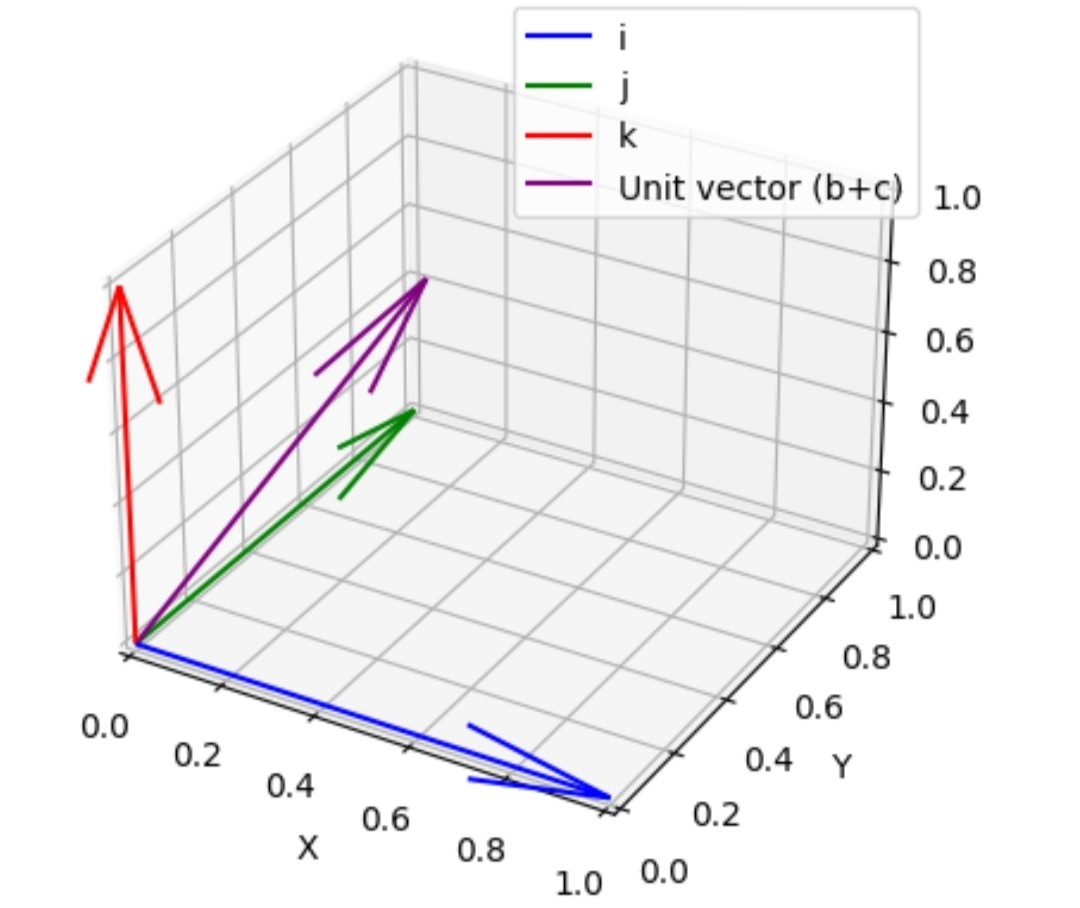
\includegraphics[width=\columnwidth]{figs/unitvector}
\caption{}
\end{center}				
\end{figure}
\end{enumerate}
\end{document}
	
